\section{Introduction}

\begin{figure*}

  \begin{panel}{(a)}{\textwidth}
    \vspace{5mm}
    \small
    \tikzsetnextfilename{figure_1_overview}
    \usetikzlibrary{spy}%
\def\blinky#1#2#3#4#5{%
  \begin{tikzpicture}[node distance=3mm]
    \node[site#1] (s1) {};
    \node[site#2,right of=s1] (s2) {};
    \coordinate (s12) at ($(s1)!.5!(s2)$);
    \node[site#3,right of=s2] (s3) {};
    \node[site#4,below of=s12] (s4) {};
    \node[site#5,right of=s4] (s5) {};
    \foreach \angle in {0, 45, 90, 135, 180, 225, 270, 315}{
      \begin{scope}[rotate=\angle]
        \draw[sitelight#1] ($(s1)+(0,0.13)$) -- ($(s1)+(0,0.16)$);
        \draw[sitelight#2] ($(s2)+(0,0.13)$) -- ($(s2)+(0,0.16)$);
        \draw[sitelight#3] ($(s3)+(0,0.13)$) -- ($(s3)+(0,0.16)$);
        \draw[sitelight#4] ($(s4)+(0,0.13)$) -- ($(s4)+(0,0.16)$);
        \draw[sitelight#5] ($(s5)+(0,0.13)$) -- ($(s5)+(0,0.16)$);
      \end{scope}
    }
  \end{tikzpicture}
}%
\begin{tikzpicture}

  \begin{scope}[spy using outlines={magnification=2,size=12mm,very thick}]

    \node[image] (frame) {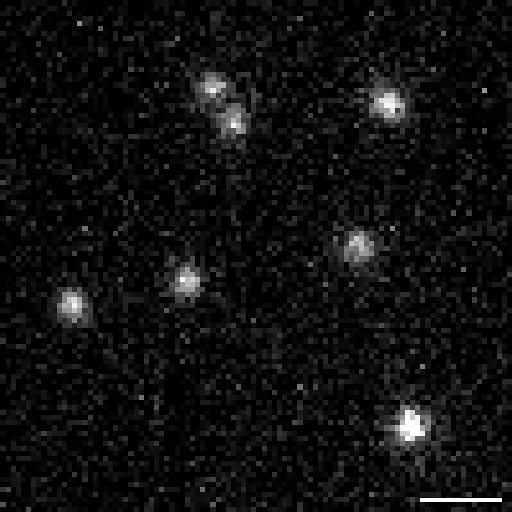
\includegraphics[width=4cm]{figures/data/overview/sample_frame}};

    \spy on ($(frame)+(1.1, 1.2)$)
      in node (patch_3) [image,right=6mm,anchor=north west]
      at (frame.north east);
    \spy on ($(frame)+(0.9, 1.1)$)
      in node (patch_2) [image,right=6mm,anchor=north west]
      at ($(frame.north east)-(0.1,0.1)$);
    \spy[
        draw=funkey_color_1,
        every spy on node/.append style={ultra thick},
        every spy in node/.append style={ultra thick},
        spy connection path={\draw[ultra thick] (tikzspyonnode) -- (tikzspyinnode);}
    ]
      on ($(frame)+(1.0, 1.2)$)
      in node (patch_1) [image,right=6mm,anchor=north west]
      at ($(frame.north east)-(0.2,0.2)$);
  \end{scope}

  % example trace
  \node[right=4mm,anchor=north west,text width=6cm,inner sep=0] (trace) at (patch_3.north east) {%
    \def\tracecsv{figures/data/overview/trace.csv}%
    \def\traceintensitycol{trace}%
    \def\nolabels{}%
    \tikzexternaldisable%
    \centerline{\begin{tikzpicture}%
  \begin{axis}[
    name=trace,
    width=0.8\textwidth,
    height=5cm,
    xlabel=frames,
    ylabel=intensity,
    enlarge x limits=false,
    xtick distance=500,
    grid=major,
    grid style={dashed},
    scaled ticks=false,
    ticklabel style={font=\small},
    legend style={nodes={scale=0.6, transform shape}},
  ]

    \addplot [
      color=tracecolor,
      mark=*,
      mark size=0.7pt,
      mark options={line width=0},
      fill opacity=0.8,
      draw opacity=0.2,
    ] table [
      col sep=comma,
      x=frames,
      y=\traceintensitycol
    ] {\tracecsv};
    \addlegendentry{intensity trace}

    \addplot [
      color=ztracecolor,
      thick
    ] table [
      col sep=comma,
      x=frames,
      y=\zcol
    ] {\tracecsv};
    \addlegendentry{inferred state}

    % remember min/max y-axis values for next plot
    \pgfplotsextra{
      \pgfmathparse{\pgfkeysvalueof{/pgfplots/ymin}}
      \global\let\ymin\pgfmathresult
      \pgfmathparse{\pgfkeysvalueof{/pgfplots/ymax}}
      \global\let\ymax\pgfmathresult
    }

  \end{axis}

  \begin{axis}[
    at={($(trace.east) + (4mm,0)$)},
    anchor=west,
    width=0.3\textwidth,
    height=5cm,
    yticklabel=\empty,
    xtick distance=0.005,
    xlabel=probability,
    grid=major,
    grid style={dashed, very thin},
    enlarge x limits={value=0.1,upper},
    scaled ticks=false,
    ymin=\ymin,
    ymax=\ymax,
    ticklabel style={font=\small},
    legend style={nodes={scale=0.6, transform shape}},
  ]

    \addplot+[
      xbar interval,
      mark=none,
      color=tracecolor,
      fill=tracecolor,
      fill opacity=0.6,
      draw=none,
    ] table [
      col sep=comma,
      y=\histbincol,
      x=\histcountcol,
    ] {\histogramcsv};
    \addlegendentry{intensity histogram}

    \addplot[
      color=intensitymodelcolor!80!black,
      thick
    ] table [
      col sep=comma,
      y=\histbincol,
      x=\modelfitcol
    ] {\histogramcsv};
    \addlegendentry{inferred model}

  \end{axis}
\end{tikzpicture}%
}%
    \tikzexternalenable%
  };
  \node[anchor=north,inner sep=0pt] at (trace.230) {\tiny time};
  \node[rotate=90,anchor=south,inner sep=1pt] at (trace.west) {\tiny intensity};

  % observed / hidden line
  \draw[gray,very thick]
    (patch_1.west|-frame.355) --
      node[pos=0,anchor=south west] {observed}
      node[pos=0,anchor=north west] {hidden}
      node[pos=0.35] (sample_1) {}
      node[pos=0.60] (sample_2) {}
      node[pos=0.96] (sample_3) {}
    (trace.east|-frame.355);

  % brace to MLE
  \draw[decorate,decoration={brace,raise=2mm}]
    (trace.north east) --
    node[pos=0.5,right=5mm,draw,rectangle,rounded corners] (mle) {\ours}
    (trace.south east);

  % posterior
  \node[anchor=north west,text width=3.6cm] (posterior) at ($(trace.north east)+(1.8,0.3)$) {%
    \def\posteriorcsv{figures/data/overview/posterior.csv}%
    \def\posteriorcol{posterior}%
    \def\noylabels{}%
    \tikzexternaldisable%
    \@ifundefined{noylabels}{}{%
  \pgfplotsset{yticklabel=\empty}%
}%
\begin{tikzpicture}%

  \def\eps{0.001}

  \begin{axis}[
    width=\textwidth,
    height=\textwidth,
    xlabel=\n,
    xlabel=$p(\n|\trace)$,
    grid=major,
    grid style={dashed, very thin},
    enlarge x limits=0.1,
    enlarge y limits=0,
    ymin=0,
    ymax=1,
    scaled ticks=false,
    ticklabel style={font=\small},
  ]

    \addplot+[
      ybar,
      bar width=1,
      mark=none,
      fill=posteriorcolor,
      fill opacity=0.6,
      draw=posteriorcolor,
      y filter/.expression={
        y < \eps ? nan : y
      },
    ] table [
      col sep=comma,
      y=\posteriorcol,
      x=n,
    ] {\posteriorcsv};

    \ifdefined\posteriorcolextra
      \addplot+[
        ybar,
        bar width=1,
        mark=none,
        fill=posteriorcolor!60!black,
        fill opacity=0.6,
        draw=posteriorcolor,
        y filter/.expression={
          y < \eps ? nan : y
        },
      ] table [
        col sep=comma,
        y=\posteriorcolextra,
        x=n,
      ] {\posteriorcsv};
    \fi

  \end{axis}

\end{tikzpicture}
%
    \tikzexternalenable%
  };
  \draw[arrow,shorten >=-8] (mle) -- (mle-|posterior.west);

  % blinky things
  \node (hidden) at (frame.330-|patch_1) {\blinky{off}{off}{off}{off}{off}};
  \node (z_sample_1) at (frame.330-|sample_1) {\blinky{on}{off}{on}{on}{off}};
  \node (z_sample_2) at (frame.330-|sample_2) {\blinky{on}{off}{on}{off}{off}};
  \node (z_sample_3) at (frame.330-|sample_3) {\blinky{on}{off}{off}{off}{off}};

  \draw[arrow] (z_sample_1) -- +(0, 2.4);
  \draw[arrow] (z_sample_2) -- +(0, 2.05);
  \draw[arrow] (z_sample_3) -- +(0, 1.7);

  \node[anchor=north,inner sep=10pt] at (hidden) {\strut$\n=5$};
  \node[anchor=north,inner sep=10pt] at (z_sample_1) {\strut$\z{}=3$};
  \node[anchor=north,inner sep=10pt] at (z_sample_2) {\strut$\z{}=2$};
  \node[anchor=north,inner sep=10pt] at (z_sample_3) {\strut$\z{}=1$};

\end{tikzpicture}

    \vspace{-2mm}
  \end{panel}

  \begin{panel}{(b)}{0.6\textwidth}
    \begin{panel}{}{\textwidth}
      \small
      \tikzsetnextfilename{figure_1_p_on_off}
      \centerline{\begin{tikzpicture}
  \node[siteoff,inner sep=4pt] (off) {};
  \node[siteon,right=2cm of off,inner sep=4pt] (on) {};
  \foreach \angle in {0, 45, 90, 135, 180, 225, 270, 315}{
    \begin{scope}[rotate=\angle]
      \draw[sitelighton,ultra thick] ($(on)+(0,0.26)$) -- ($(on)+(0,0.32)$);
    \end{scope}
  }
  \draw[arrow,shorten >=2mm,shorten <=2mm] (off) to[bend left] node[pos=0.5,above] (pon) {\pon} (on);
  \draw[arrow,shorten >=2mm,shorten <=2mm] (on) to[bend left] node[pos=0.5,below] {\poff} (off);

  \node[right=14mm of on] (re) {$\sim\poisson(\re\deltat)$};
  \draw[arrow,decorate,decoration={coil,aspect=0,segment length=6,post=curveto,post length=2mm}] ($(on.east)+(0.2,0)$) -- (re);

  %\node[parameters,anchor=south] at (re.north) {\strut$\parameterst = (\pon, \poff)$};

  \node[above=1mm of pon,gray] {transition model};
\end{tikzpicture}
}
    \end{panel}

    \vspace{4mm}
    \begin{panel}{(c)}{\textwidth}
      \small
      \hspace{4mm}
      \tikzsetnextfilename{figure_1_intensity_model}
      \begin{tikzpicture}

  \node (z) {\blinky{on}{off}{on}{on}{off}};
  \node[var,right=18mm of z] (c) {$\photons$};
  \node[annotation,below of=c] (c_dist) {$\sim\poisson((\z{}\re + \rb)\deltat)$};
  \draw (c) -- (c_dist);
  \draw[arrow,decorate,decoration={coil,aspect=0,segment length=6,post=curveto,post length=3mm}]
    (z.east) -- (c);

  \node[right=12mm of c,inner sep=0,yshift=2mm] (camera) {
    \tikz[plane x={(0.8,-0.4)},canvas is plane,transform shape]{
      \draw[gray,step=0.25] (0, 0) grid (1, 1);
      \node[anchor=south,gray] at (0.5, 1.1) {detector};
    }
  };

  \coordinate (camera_center) at (camera.center|-c);
  \draw[arrow,shorten >=3mm] (c) -- (camera_center);
  \node[observation,right=18mm of camera_center] (x) {$\x{}$};
  \node[annotation,below of=x] (x_dist) {$\sim\mathcal{N}(\photons\camgain + \camoffset, \camvar)$};
  \draw (x) -- (x_dist);
  \draw[arrow] (camera.east|-c) -- (x);
  \node[below=1mm of z] {\z{}};

  % parameter collections
  %\node[parameters,anchor=south west] at (z.north east) {\strut$\parameterse = (\re, \rb)$};
  %\node[parameters,anchor=south east] at (z.north-|x_dist.east) {\strut$\parametersc = (\camgain, \camoffset, \camvar)$};

  % annotations
  \node[above=2mm of c,gray] {\strut emission model};
  \node[above=2mm of x,gray] {\strut camera model};
\end{tikzpicture}

    \end{panel}
  \end{panel}
  \begin{panel}{(d)}{0.35\textwidth}
    \small
    \vspace{4mm}
    \hspace{4mm}
    \tikzsetnextfilename{figure_1_model}
    \centerline{\begin{tikzpicture}

  % parameters
  \node[var] (n) {\n};
  \node[var,below of=n] (theta_T) {\parameterst};
  \node[var,below of=theta_T] (theta_E) {\parameterse};
  \node[var,below of=theta_E] (theta_C) {\parametersc};

  % hidden states
  \node[state,right=1cm] (z1) at ($(n)!.5!(theta_T)$) {\z{1}};
  \node[state,right=4mm of z1] (z2) {\z{2}};
  \node[state,right=1cm of z2] (zt) {\z{t}};
  \node at ($(z2)!.5!(zt)$) {$\cdots$};

  % observations
  \node[observation,right=1cm] (x1) at ($(theta_E)!.5!(theta_C)$) {\x{1}};
  \node[observation,right=4mm of x1] (x2) {\x{2}};
  \node[observation,right=1cm of x2] (xt) {\x{t}};
  \node at ($(x2)!.5!(xt)$) {$\cdots$};

  % plates
  \begin{pgfonlayer}{background}
    \node[plate,fit=(z1)(zt)] (hidden) {};
    \node[plate,fit=(x1)(xt)] (observed) {};
  \end{pgfonlayer}

  % dependencies
  \draw[arrow] (n) to (hidden);
  \draw[arrow] (theta_T) to (hidden);
  \draw[arrow] (theta_E) to (observed);
  \draw[arrow] (theta_C) to (observed);
  \draw[arrow] (z1) to (x1);
  \draw[arrow] (z2) to (x2);
  \draw[arrow] (zt) to (xt);
  \draw[arrow] (z1) to (z2);
  \draw[arrow,shorten <=20] (z2) to (zt);
  \draw[shorten >=22] (z2) to (zt);

  % annotation
  \node[below of=observed] {$p(\trace|\n,\parameterst,\parameterse,\parametersc)$};

\end{tikzpicture}
}
  \end{panel}

  \caption{
      \panelref{a} Overview of the blinx method (scale bar: 1 $\mu$m)
      %
      \panelref{b} TODO
      %
      \panelref{c} TODO
      %
      \panelref{d} TODO \ours is based on a Hidden Markov Model who's
      parameters are optimized to build the final posterior distribution
  }
  \label{fig:method:overview}
\end{figure*}


% FLIP this first paragraph
Fluorescence microscopy has advanced understanding of biological systems by providing precise localization information 
  of molecular species, but its ability to determine quantitative information, such as molecular counts remains limited.
  %
  For large structures, such as whole cells or organelles, individual objects can be spatially separated, 
  and counting becomes trivial.
  %
  However, due to the diffraction limit, standard fluorescent imaging methods are limited to a resolution of 200 nm and 
  individual objects smaller than this threshold can no longer be separated.
  %
  The development of super-resolution techniques \cite{betzig_2006, rust_2006}, has surpassed the diffraction limit, and allows
  for the spatial separation of objects as close as 10 nm apart \cite{valli_seeing_2021}.
  %
  However, many objects of interest are smaller still, or physically positioned closer 
  together and cannot be spatially separated even with super-resolution techniques.

% Examples of importance to biology
Molecular counting aims to determine the absolute number of subunits
  associated in a complex, a quantity that is often essential to understanding the
  underlying biology of a system. 
  %
  Here are three examples:
  \begin{itemize}
  
    \item Immune response: the activation of T cells is sensitive to single ligands, and quantifying 
      the molecular count of ligand - receptor interactions informs understanding of downstream signalling pathways and sensitivity~\cite{irvine_2002}.

    \item TGF-$\beta$ signaling: the function of Smad is dependant on its oligomeric state \cite{inman_2002, moustakas_2002}. Determining the relative 
      amounts of monomeric, and trimeric states, though molecular counting, informs understanding of pathway activity.

    \item GPCRs signaling: G-protein coupled receptors exist as monomers, dimers, or higher order oligomers, 
      and again downstream signalling is dependant on oligomeric state~\cite{felce_2018, breitwieser_2004}.
      Quantifying molecular count of these oligomers would inform understanding of the signalling state of the cell.

    \end{itemize}
    % Motivate fluorescence based methods
    Although other methods exist to quantify molecular count at this scale, a robust, accurate, % needs citations
    fluorescence based method would make quantification much more accessible, while maintaining the benefits
    of fluorescence imaging, such as spatial localization.

% Related work
% fluorescence intensity based counting
Perhaps the simplest method of molecular counting is correlating fluorescent
  intensity with the number of \smallobjects \cite{schmied_2012, tolar_2005}, \ie the brighter the spot is, the more there are.
  %
  This method works well for qualitative measures, but due to the noise in intensities 
  measured from any single fluorophore, lacks the precision needed to report exact counts.
  % Other methods work by separating things out in time
  In order to extract more information from the system for a more reliable count, other methods, 
  in addition to intensity values, utilize temporal information.
  % FCS and bSOFI
  Methods such as fluorescence correlation spectroscopy (FCS) \cite{otsuka_2023, wachsmuth_2015, politi_2018} and 
  balanced super-resolution optical fluctuation imaging (bSOFI) \cite{geissbuehler_2012}
  fit higher order statistics to fluctuations in fluorescent intensity over time to estimate the molecular count.
  % Bleaching based
  In other methods, temporal variation in intensity can be induced, rather than just random, \ie
  counting, by measuring the number of distinct bleaching steps observed \cite{ulbrich_2007, jain_2011, hummert_2021}.
  % PALM and STORM based
  Methods have also been developed based on the blinking fluorophores \cite{rollins_stochastic_2015, nino_2017} 
  such as those used in PALM \cite{sengupta_pcPALM_2011, lee_counting_2012} and STORM~\cite{patel_blinking_2021}. 
  % Some of these methods are also based on HMMs, should we mention that here?
  The known blinking behavior allows for more precise models than the random fluctuations measured in FCS and bSOFI, while the 
  repeated transitions in intensity provide more information than the irreversible switch in bleaching based counting.
  % Limitations
  A major limitation of these methods is the effect of photo-bleaching, as this limits the amount of time
  a single fluorophore can be observed, and makes it difficult to differentiate blinking from photo-bleaching.


% DNA-PAINT is extra useful because its emitters dont bleach either
In contrast, DNA-PAINT \cite{schnitzbauer_2017} is a method of producing blinking fluorescence that is functionally
    immune to photo-bleaching due to the continuous replenishment of fluorophores from solution \cite{stehr_2021}.
    % lbFCS
    Localization based FCS (lbFCS) \cite{stein_2019, stein_2021}, combines the structured blinking of DNA-PAINT, with the 
    principles of FCS, fitting the autocorrelation function of intensity over time to produce a count,
    and is able to count up to 6 molecules in a single diffraction limited spot.
    % qPAINT
    Quantitative DNA-PAINT (qPAINT \cite{jungmann_2016}) estimates the molecular count based on the frequency of blinking events, \ie, 
    a blinking rate of 1 event per second is calibrated to 1 molecule, therefore an observation of 10 events per second
    produces a count of 10 molecules.
    % Limitations
    However, both of these methods are limited in that they fit summary statistics,
    rather than the data directly. 
    %
    Further, all of the methods mentioned provide a single estimate of molecular count.
    A well calibrated probabilistic estimate would provide 
    
% Our Model
% ----------
% fully Bayesian
We propose \ours, a fully Bayesian model to estimate the molecular 
  count directly from a fluctuating sequence of fluorescent intensity measurements over time.
  % Based on a fully differentiable markov chain
  Based on a fully differentiable Hidden Markov Model, \ours fits 7 parameters
  directly to the sequence of measurements, estimating a likelihood for each possible count. 
  % probabilistic
  These likelihoods can be directly compared, producing a posterior distribution of counts 
  given the observation sequence. 
  % more accurate than existing methods 
  \ours is validated on a series of simulated experiments, and shows a significant improvement in performance 
  over both lbFCS and qPAINT.
  %
  Finally the counting ability of \ours is proven experimentally, by validating the estimated count
  with ground truth measured by super-resolution DNA-PAINT.


